\chapter{The Canonical Ensemble}
Recall that the canonical ensemble was an ensemble of systems with the same volume, particle number and temperature. To create a canonical ensemble, we put together systems that are overall isolated together where they can exchange energy with one another. 
\begin{figure}[h!]
    \centering
\begin{tikzpicture}
    % Draw the outer box with hatching
    \fill[pattern=north east lines] (-0.5,0.5) rectangle (4.5,-4.5);
    \fill[white] (0,0) rectangle (4,-4);
    
    % Draw the grid
    \draw[thick] (0,0) grid (4,-4);
    
    % Place the text T.V.N. in each cell
    \foreach \x in {0.5,1.5} {
        \foreach \y in {-0.5, -0.5} {
            \node at (\x,\y) {\footnotesize N,V,T};
    \fill[pattern=north east lines] (2,-2) rectangle (3,-3);
    \node at (2.5,-2.5) {\LARGE\textbf{A}};
        }
    }
\end{tikzpicture}
    \caption{A canonical ensemble with adiabatic walls and a reference system $A$.}
    \label{fig:canonical_ensemble}
\end{figure}
Here we will consider a reference system that we will denote as $A$. The rest of the system (denoted $R$) then looks like a heat reservoir. The full system is isolated by adiabatic walls. Therefore, the complete system itself can be considered as part of a microcanonical ensemble. Now consider the entropy of the total system. For $\Omega$ the number of microstates in the entire system, the entropy is
\begin{equation}
    S_T = k_B\ln\Omega.
\end{equation}
If the reference system and the reservoir are weakly interacting, 
\begin{equation}
    \Omega = \Omega_A(U_A)\Omega_R(U_R) \hspace{0.5cm}\textrm{and}\hspace{0.5cm}    U_T=U_A+U_R.
\end{equation}

Now, the question is: For a given microstate of $A$, how many microstates are there in the full system?\\
To answer this, let $A$ be in a particular microstate with $E=E_i$. Then,
\begin{equation}
    \Omega_A(E_i)=1\implies\Omega_T(E_i)=\Omega_R(U_T-E_i).
\end{equation}
Temperature of the heat bath is:
\begin{equation}
    \frac{1}{T}=\lrp{\periv{S_R}{U_R}}_V\implies\frac{1}{T}=k_B\periv{}{U_R}\ln\Omega_R.
\end{equation}
Integrating this equation, we get
\begin{equation}
    \frac{U_R}{k_BT}=\ln\Omega_R+C(V)\implies\Omega_R=\gamma e^{U_R/k_BT}
\end{equation}
where $\gamma=e^{C(V)}$. Then,
\begin{equation}
    \Omega_T(E_i)=\Omega_R(U_T-E_i)\implies\Omega_T(E_i)=\gamma\exp\lrp{\frac{U_T-E_i}{k_BT}}.
\end{equation}
With this, we obtain the case for a specific microstate. For the full system:
\begin{equation}
    \Omega_T=\sum_j\Omega_T(E_j)=\gamma\sum_j\exp\lrp{\frac{U_T-E_j}{k_BT}}=\gamma e^{U_T/k_BT}\sum_je^{-E_j/k_BT}.
\end{equation}
The probability of the reference system being in the energy level $E_i$ is
\begin{equation}
    p_i=\frac{\Omega_T(E_i)}{\sum_j\Omega_T(E_j)}=\frac{\gamma e^{U_T/k_BT}e^{-E_i/k_BT}}{\gamma e^{U_T/k_BT}\sum_je^{-E_j/k_BT}}=\frac{e^{-E_i/k_BT}}{\sum_je^{-E_j/k_BT}}.
\end{equation}
Here, we define two quantities: \textbf{Inverse temperature} $\beta=\frac{1}{k_BT}$ and the \textbf{partition function} $Z=\sum_je^{-\beta E_j}$. Then,
\begin{equation}
    p_i = \frac{e^{-\beta E_i}}{Z}.
\end{equation}
If an energy level is $g_i$-fold degenerate: 
\begin{equation}
    p_i=\frac{g_ie^{-\beta E_i}}{Z}.
\end{equation}
\section{Entropy for a System in a \\ Canonical Ensemble}
    For a given total energy of the ensemble of $m$ systems, let each one be in a state $\psi_i$. Let us denote the number of states $\psi_i$ as $n_i$. The total number of ways this can be realised in the entire system is
    \begin{equation}
        \Omega=\frac{m!}{n_1!n_2!...}
    \end{equation}
    We know that the classical probability to choose a state $\psi_i$ at random is $p_i=n_i/m$. Then the entropy is
    \begin{align}
        S=k_B\ln\Omega=k_B\ln\frac{m!}{n_1!n_2!...}=k_B(\ln m!-\ln\lrp{\prod_in_i!)}= k_B\lrp{\ln m! -\sum_i\ln n_i!}
    \end{align}
    By Stirling's approximation,
    \begin{align}
        S=k_B\lrp{m\ln m-m-\sum_i^m(n_i\ln n_i-n_i)}=k_B\lrp{m\ln m-m-\sum_i^mn_i\ln n_i+\sum_i^mn_i}.
    \end{align}
    Since $\sum_i^mn_i=m$;
    \begin{equation}
        S=k_B\lrp{\sum_i^mn_i\ln m-\sum_i^mn_i\ln n_i}=k_B\sum_i^mn_i(\ln m-\ln n_i)=k_B\sum_i^mn_i\ln\frac{m}{n_i}
    \end{equation}
    Multiplying via unity by $m$;
    \begin{equation}
        S=mk_B\sum_i^m\frac{n_i}{m}\ln\frac{m}{n_i}=-mk_B\sum_i^m\frac{n_i}{m}\ln\frac{n_i}{m}.
    \end{equation}
    The entropy per system is this entropy divided by $m$. With this, we obtain the \textbf{Gibbs' definition of the entropy}.
    \begin{equation}
        S=-k_B\sum_ip_i\ln p_i
    \end{equation}
    For the specific entropy of the canonical ensemble;
    \begin{align}
        p_i=\frac{e^{-\beta E_i}}{Z}\implies & S=-k_B\sum p_i\ln\frac{e^{-\beta E_i}}{Z}=k_B\sum p_i\beta E_i +k_B\sum p_i\ln Z \notag\\
        \implies & S = k_B\beta\underbrace{\sum_ip_iE_i}_{\Bar{U}}+k_B\ln Z\underbrace{\sum_ip_i}_1.\notag\\
        \implies & S=k_B\beta\Bar{U}+k_B\ln Z = \frac{\bar{U}}{T}+k_B\ln Z\notag\\
        \implies &U-TS=-k_BT\ln Z
    \end{align}
    Recall that the Helmholtz free energy was defined as $F=U-TS$. Then,
    \begin{equation}
        F = -k_BT\ln Z.
    \end{equation}
    Free energy is minimum for a system at equilibrium where the temperature is constant. Once we know the expression for the free energy, we can obtain other thermodynamical properties.
    \begin{equation}
        dF = -SdT -PdV
    \end{equation}
    \paragraph{1) Pressure:}
    \begin{equation}
        P = -\lrp{\periv{F}{V}}_T = k_BT\lrp{\periv{\ln Z}{V}}_T
    \end{equation}
    \paragraph{2) Entropy:}
    \begin{equation}
        S = -\lrp{\periv{F}{T}}_V = k_B\lrp{\periv{T\ln Z}{T}}_V=k_B\ln Z +k_BT\lrp{\periv{\ln Z}{T}}_V=k_B\ln Z+\frac{k_BT}{Z}\periv{Z}{T}
    \end{equation}
    \paragraph{3) Heat Capacity:}
    \begin{equation}
        C_V=T\lrp{\periv{S}{T}}_V = k_BT\periv{^2}{T^2}\lrp{T\ln Z}
    \end{equation}
    \paragraph{3) Internal Energy:}
    \begin{align}
        U=&F+TS=-k_BT\ln Z - T\lrp{\periv{F}{T}}_V\notag\\
        =& -k_BT\ln Z -Tk_B\lrp{\periv{}{T}T\ln Z}_V = -k_BT\ln Z +k_BT\ln Z + \frac{k_BT^2}{Z}\lrp{\periv{Z}{T}}_V \notag\\
        =& \frac{k_BT^2}{Z}\lrp{\periv{Z}{T}}_V
    \end{align}
\section{Examples}
\subsection{Two Level System}
    Assume a single spin state with energy levels $\varepsilon_{1,2}=\pm \mu B$. Then the partition function is
    \begin{equation}
        Z = e^{-\beta\varepsilon}+e^{\beta\varepsilon}.
    \end{equation}
    This gives the free energy as
    \begin{align}
        F =& -k_BT\ln Z = -k_BT\ln\lrp{e^{-\beta\varepsilon}+e^{\beta\varepsilon}}\notag\\
        =& -\frac{1}{\beta}\ln\lrp{e^{\beta\varepsilon}\lrp{1+e^{-2\beta\varepsilon}}}=-\frac{1}{\beta}\lrp{\beta\varepsilon+\ln\lrp{1+e^{-2\beta\varepsilon}}}\notag\\
        =& -\varepsilon - \frac{1}{\beta}\ln(1+e^{-2\beta\varepsilon})
    \end{align}
    Again, from the free energy we can derive other quantities.
    \begin{equation}
        S = -\lrp{\periv{F}{T}}_V = -\periv{F}{\beta}\periv{\beta}{T} = -\periv{F}{\beta}\periv{}{T}\lrp{\frac{1}{k_BT}}=-\periv{F}{\beta}\lrp{\frac{-1}{k_BT^2}}=k_B\beta^2\periv{F}{\beta}
    \end{equation}
    Now, we calculate the derivative of the free energy with respect to $\beta$.
    \begin{align}
        \periv{F}{\beta} &= -k_B\periv{}{\beta}\lrp{T\ln Z}=-k_B\periv{}{\beta}\lrp{\frac{1}{k_B\beta}\lrp{\beta\varepsilon+\ln\lrp{1+e^{-2\beta\varepsilon}}}}\notag\\
        &=-\periv{}{\beta}\lrp{\varepsilon+\frac{1}{\beta}\ln\lrp{1+e^{-2\beta\varepsilon}}}=-\lrp{\frac{-1}{\beta^2}\ln(1+e^{-2\beta\varepsilon})-\frac{2\varepsilon e^{-2\beta\varepsilon}}{\beta(1+e^{-2\beta\varepsilon})}}
    \end{align}
    Then,
    \begin{equation}
        S = k_B\ln\lrp{1+e^{-2\beta\varepsilon}}+\frac{2k_B\beta\varepsilon}{e^{2\beta\varepsilon}+1}.
    \end{equation}
    Now, we calculate the heat capacity.
    \begin{align}
        C_V = T\lrp{\periv{S}{T}}_V = T\periv{S}{\beta}\periv{\beta}{T}=-k_B\beta^2T\periv{S}{\beta} = -\beta\periv{S}{\beta}
    \end{align}
    Again, we calculate the derivative of the entropy.
    \begin{align}
        \periv{S}{\beta} =& k_B\periv{}{\beta}\lrp{\ln(1+e^{-2\beta\varepsilon})+\frac{2\beta\varepsilon}{e^{2\beta\varepsilon}+1}} \notag\\
        =& k_B\lrb{\frac{-2\varepsilon e^{-2\beta\varepsilon}}{1+e^{-2\beta\varepsilon}}+\frac{2\varepsilon(e^{2\beta\varepsilon}+1)-2\beta\varepsilon(2\varepsilon e^{2\beta\varepsilon})}{(e^{2\beta\varepsilon}+1)^2}}\notag\\
        =& k_B\lrb{\frac{-2\varepsilon}{e^{2\beta\varepsilon}+1}+\frac{2\epsilon}{e^{2\beta\varepsilon}+1}-\beta\lrp{\frac{2\varepsilon e^{\beta\varepsilon}}{e^{2\beta\varepsilon}+1}}^2}\notag\\
        =& -k_B\beta\varepsilon^2\lrp{\frac{2}{e^{\beta\varepsilon}+e^{-\beta\varepsilon}}}^2
    \end{align}
    Therefore, the heat capacity is
    \begin{equation}
        C_V = k_B\frac{(\beta\varepsilon)^2}{\cosh^2\beta\varepsilon}.
    \end{equation}
\subsection{Particle in a 1-D and a 3-D Box}
    Recall that the eigenstates and eigenvalues of the one dimensional particle in a box problem were
    \begin{equation}
        \phi_n = \sqfrac{2}{L}\sin(k_nx) \hspace{0.5cm},\hspace{0.5cm} E_n = \alpha n^2
    \end{equation}
    where
    \begin{equation}
        k_n = \frac{n\pi}{L} \hspace{0.5cm}\mathrm{and}\hspace{0.5cm} \alpha = \frac{\hbar^2\pi^2}{2mL^2}.
    \end{equation}
    Then the partition function of the system is
    \begin{equation}
        Z = \sum_{n=1}^\infty e^{-\alpha\beta n^2} \approx \int_0^\infty dn e^{-\gamma n^2}
    \end{equation}
    where we defined $\gamma = \alpha\beta$ and used the fact that at lower limit of $n$, the conversion from the summation to integration holds approximately. This integral is a Gaussian integral which we know the solution of. 
    \begin{equation}
        Z = \frac{1}{2}\sqfrac{\pi}{\gamma}=\frac{1}{2}\sqrt{\pi k_BT\frac{2mL^2}{\pi^2\hbar^2}}=\sqrt{\frac{L^2mk_BT}{2\pi\hbar^2}}
    \end{equation}
    Here, we define a quantity called the \textbf{thermal de Broglie wavelength}.
    \begin{equation}
        \lambda_D := \sqfrac{2\pi\hbar^2}{mk_BT} \implies Z = \frac{L}{\lambda_D}
    \end{equation}
    Now let us calculate the free energy, entropy, and the heat capacity. For ease of notation, we define a constant: $A = mL^2k_B/2\pi\hbar^2$ such that $Z=\sqrt{AT}$.
    \begin{equation}
        F = -k_BT\ln Z = -k_BT\ln\sqrt{AT}=-\frac{k_BT}{2}\ln(AT)
    \end{equation}
    \begin{align}
        S = -\lrp{\periv{F}{T}}_V = \frac{k_B}{2}\lrp{\ln(AT)+\frac{T}{AT}A}=\frac{k_B}{2}(\ln(AT)+1)
    \end{align}
    \begin{equation}
        C_V = T\lrp{\periv{S}{T}}_V = \frac{k_BT}{2}\frac{A}{AT}=\frac{k_B}{2}
    \end{equation}
    Now let us consider the three dimensional particle in a box. Recall that we can think of this as three particles each in a one dimensional box. Then recall that the energies are given by
    \begin{equation}
        E_i = \frac{\hbar^2\pi^2}{2mL^2}\sum_i^3n_i^2.
    \end{equation}
    Defining a constant $\gamma=\hbar^2\pi^2/2mL^2$, we get the partition function as
    \begin{equation}
        Z = \sum_{n_1}^\infty\sum_{n_2}^\infty\sum_{n_3}^\infty e^{-\gamma\beta(n_1^2+n_2^2+n_3^2)} = \sum_{n_1}^\infty e^{-\gamma\beta n_1^2}\sum_{n_2}^\infty e^{-\gamma\beta n_2^2}\sum_{n_3}^\infty e^{-\gamma\beta n_3^2}.
    \end{equation}
    We have already calculated these sums via the Gaussian integral in the one dimensional case. We know that each of the sums contribute a factor of $L/\lambda_D$ to the partition function giving us
    \begin{equation}
        Z = \lrp{\frac{L}{\lambda_D}}^3 = V\lrp{\frac{mk_BT}{2\pi \hbar^2}}^{3/2}.
    \end{equation}
    Then the free energy and entropy are:
    \begin{equation}
        F = -k_BT\ln\lrb{V\lrp{\frac{mk_BT}{2\pi\hbar^2}}^{3/2}}=-k_BT\ln V-\frac{3k_BT}{2}\ln\frac{mk_BT}{2\pi\hbar^2},
    \end{equation}
    \begin{equation}
        S =  k_B\ln V + \frac{3k_B}{2}\ln\frac{mk_BT}{2\pi\hbar^2}+\frac{3k_BT}{2}\frac{2\pi\hbar^2}{mk_BT}\frac{mk_B}{2\pi\hbar^2} = k_B\ln V + \frac{3k_B}{2}\lrp{1+\ln(AT)}.
    \end{equation}
    Note that this entropy has the same form as the entropy in the one dimensional case where they only differ by the definition of the constant $A$. Therefore, the heat capacity will be similar to the one dimensional case.
    \begin{equation}
        C_V = T\lrp{\frac{3k_B}{2}\frac{A}{AT}} = \frac{3k_B}{2}
    \end{equation}
    Finally, let us look at the pressure: 
    \begin{equation}
        P = -\lrp{\periv{F}{V}}_T = \frac{k_BT}{V}.
    \end{equation}
    Note that this is the ideal gas law for $N=1$. For $N$ particles, we get: $PV=Nk_BT$. However, one must note that while $C_V$ can simply be multiplied by $N$, $F$ and $S$ cannot. For $N$-particle systems, $Z$ must be calculated for $N$-particles.
\newpage
\section{First Law of Thermodynamics}
    Question: What happens to the energy levels and probabilities if heat is added or work is done on the system? To answer this, let us write the internal energy of the system. 
    \begin{equation}
        U = \sum_ip_iE_i \hspace{0.5cm}\mathrm{where}\hspace{0.5cm} p_i=\frac{e^{-E_i/k_BT}}{Z}
    \end{equation}
    Then, $dU = \sum_iE_idp_i + \sum_ip_idE_i$. Doing work on the system requires changing the constraints on the system such as the volume, electric field and so on. Note that, since the energy $E_i$ depends on these quantities and not $p_i$, changing these will cause a change $dE_i$ in the energy. Therefore, the work must be related to the second term in Equation (5.5.2).
    \begin{align}
        \implies & \dbar W = \sum_ip_idE_i \\
        \implies & \dbar Q = \sum_iE_idp_i
    \end{align}
    In short, doing work changes the energy levels while adding heat changes the probabilities. 

    \begin{problem}{What is the work done on a particle in a three dimensional box when the volume of the box is shrunk? Assume non-interacting particles. }
     a
        \begin{equation}
            \varepsilon_n = \frac{\hbar^2\pi^2}{2mL^2}n^2 = \frac{\hbar^2\pi^2}{2mV^{2/3}}n^2 \implies \periv{\varepsilon_n}{V} = -\frac{2}{3}V^{-5/3}\frac{\pi^2\hbar^2}{2m}n^2 = -\frac{2}{3}\frac{\varepsilon_n}{V}
        \end{equation}
        Considering non-interacting particles, the total energy is 
        \begin{equation}
            E = \sum_mn_m\varepsilon_m
        \end{equation}
        where $n_m$ is the occupation number of the mth level. Then the volume derivative of the total energy is
        \begin{equation}
            \periv{E}{V} = \sum_mn_m\periv{\varepsilon_m}{V} = -\frac{2}{3V}\sum_mn_m\varepsilon_m = -\frac{2E}{3V}.
        \end{equation}
        Now consider mechanical work done on the system.
        \begin{equation}
            -PdV = \sum_ip_idE_i = \sum_ip_i\periv{E_i}{V}dV = -\frac{2}{3}\sum_ip_i\frac{E_i}{V}dV = \frac{-2}{3}U\frac{dV}{V}
        \end{equation}
        \begin{equation}
            \therefore U = \frac{3}{2}PV
        \end{equation}
        On the other hand, from the ideal gas law: $PV=Nk_BT$
        \begin{equation}
            \therefore U = \frac{3}{2}Nk_BT
        \end{equation}
        This is the kinetic theory result for the internal energy of an ideal gas. 
    \end{problem}
\section{Rotational and Vibrational \\ Degrees of Freedom}
    
    \begin{wrapfigure}{l}{0.4\textwidth}
        \centering
        \resizebox{0.3\textwidth}{!}{%
        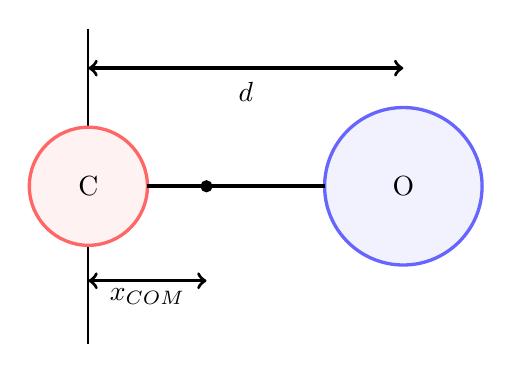
\begin{tikzpicture}[]
            \draw[black, thick] (0,4) -- (0,0);
            \filldraw[color=red!60, fill=red!5, very thick](0,2) circle (0.75);
            \filldraw[color=blue!60, fill=blue!5, very thick](4,2) circle (1);
            \draw[black, ultra thick] (0.75,2) -- (3,2);
            \filldraw [black] (1.5,2) circle (2pt);
            \node[black] at (0,2)  {C};
            \node[black] at (4,2) {O};
            \draw[black,very thick, <->] (0, 0.8) -- (1.5,0.8);
            \draw[black, very thick, <->] (0,3.5) -- (4, 3.5);
            \node[black] at (2, 3.2) {$d$};
            \node[black] at (0.75, 0.6) {$x_{COM}$};
        \end{tikzpicture}
        }
        \caption{A diatomic molecule}
        \label{fig:diatomic}
    \end{wrapfigure}
    Consider a diatomic molecule. When working on the rotational degrees of freedom, we will use two parameters: The position of the centre of mass $x_{COM}$ and the moment of inertia of the molecule around the center of mass $I_{COM}$. The position of the centre of mass is given by $x_{COM} = \frac{m_O}{m}d$ where $m$ is the total mass of the system: $m = m_O + m_C$. The moment of inertia is calculated as\\
    \begin{align}
        I_{COM} =& m_O(d-x_{COM})^2+m_Cx_{COM}^2 = m_O\lrp{d-\frac{m_Od}{m}}^2+m_C\lrp{\frac{m_Od}{m}}^2 \notag \\
        =& m_Od^2\lrp{\frac{m-m_O}{m}}^2+\frac{m_Cm_O^2d^2}{m^2} = \frac{m_Om_C^2d^2}{m^2}+\frac{m_Cm_O^2d^2}{m^2}\notag \\
        =& \frac{m_Cm_Od^2(m_O+m_C)}{m^2} = \frac{m_Cm_O}{m}d^2 = \mu d^2
    \end{align}
    where we defined the reduced mass $\mu = \frac{m_Cm_O}{m}$. From this, we can calculate the rotational energy: $L^2/2I$. Translating this into quantum mechanical variables, we get $\hat{H} = \frac{\hat{L}^2}{2I}$.
    The eigenfunctions of the squared angular momentum operator are the spherical harmonics $Y_l^m$ with eigenvalues $\varepsilon_l = \frac{\hbar^2 l(l+1)}{2I}$ with $(2l+1)$-fold degeneracy. Then the partition function is:
    \begin{equation}
        Z = \sum_l(2l+1)\exp\lrp{-\beta\frac{\hbar^2l(l+1)}{2I}}.
    \end{equation}
    Now, let us consider the limits: \\
    $T\to0\implies\beta\to\infty$: As $\beta\to0$, the exponential will decay to 0. Then we can truncate the sum at some $l$. Let us take only to $l=1$ and get $Z = 1 + 3\exp\lrp{-\frac{\hbar^2}{k_BTI}}$.
    Calculating the thermodynamical quantities:
    \begin{equation}
        F = -k_BT\ln Z = -k_BT\ln\lrp{1+3e^{-\hbar^2/k_BTI}} \approx -3k_BTe^{-\hbar^2/k_BTI}
    \end{equation}
    \begin{equation}
        S = -\periv{F}{T} = 3k_Be^{-\hbar^2/k_BTI} + 3k_BTe^{-\hbar^2/k_BTI}\lrp{\frac{\hbar^2}{k_BIT^2}} = 3k_Be^{-\hbar^2/k_BTI}\lrp{1+\frac{\hbar^2}{k_BTI}}
    \end{equation}
    \begin{align}
        C_V =& T\periv{S}{T} = 3k_BT\lrp{\frac{\hbar^2}{k_BT^2I}e^{-\hbar^2/k_BTI}\lrp{1+\frac{\hbar^2}{k_BTI}}-\frac{\hbar^2}{k_BT^2I}e^{-\hbar^2/k_BTI}}\notag\\
        =& \frac{3\hbar^4}{k_BI^2T^2}e^{-\hbar^2/k_BTI}
    \end{align}
    Now consider the $T\to\infty$ limit. Since the partition function will vary slowly at lower $l$, we can convert the sum into an integral.
    \begin{equation}
        Z\approx\int_0^\infty dl(2l+1)\exp\lrp{-\frac{\hbar^2l(l+1)}{2Ik_BT}} =\frac{2Ik_BT}{\hbar^2}=AT
    \end{equation}
    Then the free energy, entropy, and the heat capacity are
    \begin{equation}
        F = -k_BT\ln AT \implies S=k_B\ln AT + k_B \implies C_V = \frac{k_B}{T}.
    \end{equation}
    \begin{figure}[h!]
        \centering
        \resizebox{0.35\textwidth}{!}{%
        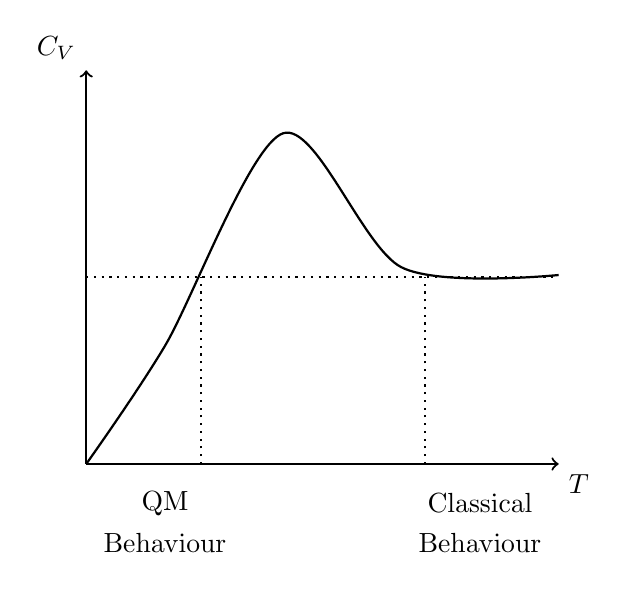
\begin{tikzpicture}
    % Axes
        \draw[thick,->] (0,0) -- (6,0) node[anchor=north west] {$T$};
        \draw[thick,->] (0,0) -- (0,5) node[anchor=south east] {$C_V$};
    
        % Horizontal dotted line
        \draw[dotted, thick] (0,2.37) -- (6,2.37);
        
        % Curve
        \draw[thick] plot[smooth] coordinates {(0,0) (1,1.5) (2.5,4.2) (4,2.5) (6,2.4)};
        
        % Dotted vertical lines
        \draw[dotted, thick] (1.46,0) -- (1.46,2.37);
        \draw[dotted, thick] (4.3,0) -- (4.3,2.37);
        
        % Labels
        \node at (1,-0.5) {QM};
        \node at (1,-1) {Behaviour};
        \node at (5,-0.5) {Classical};
        \node at (5,-1) {Behaviour};
        \end{tikzpicture}
        }
        \caption{$C_V$ plot showing the quantum mechanical and classical regions}
        \label{fig:cvrot}
    \end{figure}
    
    Now, we look at the vibrational degrees of freedom. For the vibrational motion, we observe a harmonic oscillator behaviour. The quantum mechanical harmonic oscillator has energies
    \begin{equation}
        \varepsilon_n = \hbar\omega(n+1/2).
    \end{equation}
    Therefore, the partition function is
    \begin{equation}
        Z = e^{-\hbar\omega\beta/2}\sum_{n=0}^\infty e^{\hbar\omega\beta n} = e^{-\hbar\omega\beta/2}\sum_{n=0}^\infty \lrp{e^{\hbar\omega\beta}}^n.
    \end{equation}
    This is a geometric series converging to
    \begin{equation}
        Z = \frac{e^{-\hbar\omega\beta/2}}{1-e^{\hbar\omega\beta}}.
    \end{equation}
    We again look at the low and high temperature limits:\\
    At low temperatures, the heat capacity is exactly
    \begin{equation}
        C_V=k_b(\hbar\omega\beta)^2\frac{e^{\hbar\omega\beta}}{(e^{\hbar\omega\beta}-1)^2}
    \end{equation}
    which at low temperature (high $\beta$) limit gives
    \begin{equation}
        C_V=k_B\frac{\hbar\omega\beta}{e^{\hbar\omega\beta}}.
    \end{equation}
    At high temperatures, $\hbar\omega\beta<<1$. Then,
    \begin{align}
        Z =& \frac{1}{e^{\hbar\omega\beta/2}-e^{-\hbar\omega\beta/2}}=\frac{1}{1+\frac{\hbar\omega\beta}{2}-1+\frac{\hbar\omega\beta}{2}} = \frac{k_BT}{\hbar\omega}, \\
        F =& -k_BT\ln\frac{k_BT}{\hbar\omega} = -k_BT\ln AT, \\
        S =& k_B\ln AT + k_B, \\
        C_V =& k_B.
    \end{align}
    Therefore, the total heat capacity is
    \begin{equation}
        C_V=\frac{3}{2}Nk_B + Nk_B + Nk_B.
    \end{equation}
    One must note that these degrees of freedom do not activate simultaneously. Initially (at low temperature), we only have translational degrees of freedom as the effects from the rotational and vibrational degrees of freedom die out. Then, the rotational effects are activated. At high temperatures, we have the total contribution. The activation temperatures in the case of the heat capacity are
    \begin{equation}
        T_{\mathrm{rot}} \approx \frac{\hbar^2}{2Ik_B} \hspace{0.5cm}\mathrm{and}\hspace{0.5cm}T_\mathrm{vib}\approx\frac{\hbar\omega}{k_B}
    \end{equation}
    Now, a question is: How does one calculate the partition function for continuous energy spectra, i.e. the classical limit?
    \subsection{Phase Space Representation}
        Recall that the Hamiltonian is a function of generalised coordinates and momenta. For $N$-particles, $H=H(p^N,q^N)$. Let us assume that the phase space is divided into a coarse grid with each grid having an area $\Delta A_i = \Delta x\Delta p$. The smallest area possible is $h$ due to the Heisenberg's uncertainty principle. Then, the number of states in $\Delta A_i$ is $g_i = \Delta x\Delta p / h$. This gives the partition function as
        \begin{equation}
            Z = \sum_i\frac{\Delta x\Delta p}{h}e^{-\beta E(x_i,p_i)}.
        \end{equation}
        As $\Delta x, \Delta p\to0$, we get the continuum limit: $E(x_i,p_i)\to E(x,p)$ and $\Delta x\Delta p\to dxdp$. Then,
        \begin{equation}
            Z = \frac{1}{h}\int\int dxdp_xe^{-\beta E(x,p_x)}.
        \end{equation}
        For a single particle in three dimensions, we integrate over each degree of freedom, giving us 6 integrals. 
        \begin{equation}
            Z=\frac{1}{h^3}\underbrace{\int\cdots\int}_6 d^3rd^3pe^{-\beta E(\v{r},\v{p})}
        \end{equation}
        Similarly, for $N$-particles in three dimensions, we get $6N$-integrals.
        \begin{equation}
            Z= \frac{1}{h^{3N}}\underbrace{\int\cdots\int}_{6N} d^{3N}rd^{3N}pe^{-\beta E(\v{r}_1,...,\v{r}_N,\v{p}_1,...,\v{p}_N)}
        \end{equation}
        
\section{Equipartition Theorem}
    Consider a general energy expression $E(p,q)=aq^2+bp^2$ where $a,b\in\mathbb{R}$. 
    \begin{equation}
        Z = \frac{1}{h}\int_{-\infty}^\infty dq\int_{-\infty}^\infty dp e^{-\beta(aq^2+bp^2)}=\frac{1}{h}\int_{-\infty}^\infty dq e^{-\beta aq^2}\int_{-\infty}^\infty dpe^{-\beta bp^2}
    \end{equation}
    This is a Gaussian integral giving us $Z=\frac{\pi k_BT}{h\sqrt{ab}}$. Then for $A = \frac{\pi k_B}{h\sqrt{ab}}$,
    \begin{equation}
        F = -k_BT\ln AT \hspace{1cm} S = k_B(\ln AT+1)\hspace{1cm}C_V=k_B.
    \end{equation}
    If we set $a=0$, we need to limit the position integral to a finite range to stop the partition function from diverging. 
    \begin{equation}
        Z = \frac{1}{h}\int_{-\Delta q/2}^{\Delta q/2}dq\int_{-\infty}^\infty dp e^{-\beta bp^2}=\frac{\Delta q}{h}\sqfrac{\pi}{b\beta}
    \end{equation}
    From this, we get $C_V=k_B/2$. This observation leads to the \textbf{equipartition theorem.}
    \begin{theorem}{Equipartition Theorem}
        aEvery degree of freedom that contributes a quadratic term of position or momentum to the total energy, has an average energy of $k_BT/2$ and gives a factor of $k_B/2$ to the heat capacity.
    \end{theorem}
    One can show that the Helmholtz free energy is minimised when the temperature and volume are kept constant. To prove this, we use the second law of thermodynamics: $\delta Q / T \leq \delta S$.
    \begin{equation}
        F=U-TS \implies \delta F = \delta U - T\delta S - S\delta T = \delta Q -P \delta V -T\delta S -S\delta T
    \end{equation}
    \begin{equation}
        \implies \delta F = (\delta Q -T\delta S) - P\delta V - S\delta T
    \end{equation}
    The minimum of the term in the parenthesis is 0 as stated by the second law. Then, $\delta F$ is zero when $\delta V$ and $\delta T $ are zero. 
\newpage
\section{Exercises}
    \begin{eocproblem*}{}{Each molecule in a dilute gas has an electric dipole moment of magnitude $D$. When an electric field of intensity $\varepsilon$ along the z-axis is turned on, the Hamiltonian is \begin{equation}
        H = \frac{1}{2I}p_\theta^2+\frac{1}{2I\sin^2\theta}p_\phi^2-D\varepsilon\cos\theta.
    \end{equation}
    Calculate the partition function.}
\end{eocproblem*}
        Using the Jacobian, the volume element is $dV = drd\theta d\phi dp_rdp_\theta dp_\phi$. Since $r$ is constant, we get $dV=d\theta d\phi dp_\theta dp_\phi$. Then,
        \begin{align}
            Z =& \frac{1}{h^2}\int_{-\infty}^\infty dp_\theta e^{-\beta p_\theta^2/2I}\int_0^\pi d\theta e^{\beta D\varepsilon\cos\theta}\int_{-\infty}^\infty dp_\phi e^{-\beta p_\phi^2/2I\sin^2\theta}\int_0^{2\pi} d\phi \notag\\
            =& \sqfrac{2\pi I}{\beta}\frac{2\pi}{h^2}\sqfrac{2\pi I}{\beta}\int_0^\pi d\theta \sqrt{\sin^2\theta}e^{\beta D\varepsilon\cos\theta}.
        \end{align}
        From $0$ to $\pi$, $\sqrt{\sin^2\theta}=\sin\theta$. Then,
        \begin{equation}
            Z = \frac{4\pi^2I}{\beta h^2}\int_0^\pi d\theta \sin\theta e^{\beta D\varepsilon \cos\theta} = \frac{4\pi^2I}{\beta h^2} \int_\pi^0d(\cos\theta)e^{\beta D\varepsilon\cos\theta} = \frac{4\pi^2I}{\beta h^2} \frac{e^{\beta D\varepsilon \cos\theta}}{\beta D \varepsilon}\bigg\vert_\pi^0
        \end{equation}
        \begin{equation}
            Z = \frac{8\pi^2I}{\beta^2h^2D\varepsilon}\frac{e^{\beta D\varepsilon}-e^{-\beta D\varepsilon}}{2} = \frac{8\pi^2I}{\beta^2h^2D\varepsilon}\sinh(\beta D\varepsilon)
        \end{equation}


    \begin{eocproblem*}{5.17 from Bowley \& Sanchez}
        {
        The partition function for an interacting gas is assumed to be
        \[
        Z = \left( \frac{V - Nb}{N} \right)^N \left( \frac{mk_BT}{2\pi \hbar^2} \right)^{3N/2} e^{N^2 a^2 / V k_B T}
        \]
        where \(a\) and \(b\) are constants. Show that the pressure is of the same form as van der Waals equation. Calculate the internal energy.}
    \end{eocproblem*}
        \begin{equation}
        F = U - TS = -k_B T \ln Z
        \end{equation}
        \begin{equation}
        dF = dU - TdS - SdT = TdS - PdV - TdS - SdT = -PdV - SdT
        \end{equation}
        \begin{equation}
        P = - \left( \frac{\partial F}{\partial V} \right)_T , S = - \left( \frac{\partial F}{\partial T} \right)_V
        \end{equation}
        \begin{equation}
        F = -k_B T \left[ N \ln \left( \frac{V - Nb}{N} \right) + \frac{3N}{2} \ln \left( \frac{mk_B T}{2\pi \hbar^2} \right) + \frac{N^2 a^2}{V k_B T} \right]
        \end{equation}
        \begin{equation}
        F = -Nk_B T \left[ \ln (V - Nb) - \ln N + \frac{3}{2} \ln \left( \frac{mk_B }{2\pi \hbar^2} \right) + \frac{3}{2}\ln T + \frac{N a^2}{V k_B T} \right]
        \end{equation}
        \begin{equation}
        P = - \left( \frac{\partial F}{\partial V} \right)_T = \frac{Nk_B T}{V - Nb} - \frac{N^2 a^2 k_B T}{V^2 k_B T}
        \end{equation}
        which is of the form of van der Waals equation
        \begin{equation}
        \left[ P + \frac{aN^2}{V^2} \right] (V - Nb) = Nk_B T.
        \end{equation}
        \begin{equation*}
            \begin{split}
                U = F + TS =  -Nk_B T \left[ \ln (V - Nb) - \ln N + \frac{3}{2} \ln \left( \frac{mk_B }{2\pi \hbar^2} \right) + \frac{3}{2}\ln T + \frac{N a^2}{V k_B T} \right]
        \\
            +Nk_B T \left[ \ln (V - Nb) - \ln N + \frac{3}{2} \ln \left( \frac{mk_B }{2\pi \hbar^2} \right) + \frac{3}{2}\ln T\right] + N k_B \frac{3}{2}T
            \end{split}
        \end{equation*}
        \begin{equation}
            U = -\frac{N^2a^2}{V}+\frac{3}{2} Nk_B T
        \end{equation}

        \begin{eocproblem*}{5.21 from Bowley\& Sanchez}
            {By putting $\beta = 1/k_B T$, write $Z = \sum_i e^{-\beta E_i}$, and show that
            \begin{enumerate}[label=(\alph*)]
            \item \begin{equation*}
                -\left(\frac{\partial \ln Z}{\partial\beta}\right) = \sum_i p_i E_i = \Bar{U}
            \end{equation*}
            \item Consider the second derivative of $\ln Z$ with respect to $\beta$. Show that
             \begin{equation*}
                 \left(\frac{\partial^2 \ln Z}{\partial\beta^2}\right) = \sum_i E_i^2 \frac{e^{-\beta E_i}}{Z} - \left(\sum_i E_i \frac{e^{-\beta E_i}}{Z}\right)^2 =\sum_i E_i^2 p_i - \Bar{U}^2 .
            \end{equation*}
            \item Standard deviation in energy is given by:
            \begin{equation*}
                \Delta U^2=\left(\frac{\partial^2 \ln Z}{\partial\beta^2}\right).
            \end{equation*}
            \item The average internal energy of harmonic oscillator is:
            \begin{equation*}
                \Bar{U}=\frac{\hbar\omega}{2}+\frac{\hbar\omega}{e^{\hbar\omega/k_BT}-1}.
            \end{equation*}
            \item Calculate the average internal energy and the standard deviation in energy for a two-level system with energies $\varepsilon$ and $-\varepsilon$.
            \end{enumerate}
            }
        \end{eocproblem*}
            \begin{enumerate}[label=(\alph*)]
            \item \begin{equation}
                \beta =\frac{1}{k_BT}\quad,\quad F=-k_BT\ln Z =-\frac{1}{\beta}\ln\left(\sum_i e^{-\beta E_i}\right) = \Bar{U} -TS
            \end{equation}
            
            Then,
            \begin{equation}
            \frac{\partial\beta}{\partial T}  = -\beta^2 k_B = -\frac{1}{k_BT^2}.
            \end{equation}
            \begin{align}
                 S =& - \left(\frac{\partial F}{\partial T} \right)_V = \left(\frac{\partial F}{\partial \beta} \right)_V \left(\frac{\partial \beta}{\partial T} \right)_V \notag
                 \\
                 =&-\left[\frac{1}{\beta^2}\ln Z - \frac{1}{\beta} \left(\frac{\partial \ln Z}{\partial \beta} \right) \right] (-\beta^2 k_B)\notag 
                 \\
                 =& k_B \ln Z -\beta k_B \left(\frac{\partial \ln Z}{\partial \beta} \right)
            \end{align}
            
            \begin{equation}
                F=\Bar{U}-TS \quad \implies \quad \Bar{U} = F+TS 
            \end{equation}
            \begin{equation}
            \Bar{U} = -k_BT\ln Z +T\left[k_B \ln Z -\beta k_B \left(\frac{\partial \ln Z}{\partial\beta} \right)\right]
            \end{equation}
            
            \begin{equation}
                \Bar{U} = -\left(\frac{\partial \ln Z}{\partial\beta} \right)=\sum_i p_i E_i
            \end{equation}
            
            or,
            \begin{equation}
            \begin{split}
            \left(\frac{\partial \ln Z}{\partial\beta} \right)=\frac{\partial}{\partial\beta}\ln\sum_i e^{-\beta E_i} = \frac{\sum_i -E_i e^{-\beta E_i}}{\sum_j -e^{-\beta E_j}}
            \\
            =\frac{\sum_i -E_i e^{-\beta E_i}}{Z} = =\sum_i\frac{ -E_i e^{-\beta E_i}}{Z} = -\sum_i p_i E_i = -\Bar{U}
            \end{split}
            \end{equation}
            \item 
            \begin{equation*}
                \frac{\partial^2}{\partial \beta^2} \ln Z = \frac{\partial^2}{\partial \beta^2} \ln \sum_i e^{-\beta E_i} = \frac{\partial}{\partial \beta} \left[\frac{\sum_i -E_i e^{-\beta E_i}}{\sum_i e^{-\beta E_i}}\right] 
                    \end{equation*}
                    \begin{equation}      
                    = -\frac{\partial}{\partial  \beta} \sum_i p_i E_i = -\sum_i \frac{\partial p_i}{\partial \beta}E_i - \sum_i p_i \frac{\partial E_i}{\partial \beta} = -\sum_i E_i \frac{\partial}{\partial \beta} \left(\frac{e^{\beta E_i}}{Z}\right)
                    \end{equation}
                    \begin{equation*}
                    = -\sum_i E_i e^{\beta E_i} \frac{-E_i Z-\frac{\partial Z}{\partial \beta}}{Z} = \sum_i E_i e^{\beta E_i} \frac{1}{Z}+\sum_i E_i e^{\beta E_i} \frac{1}{Z^2}\frac{\partial Z}{\partial \beta}
            \end{equation*}
            \begin{equation*}
                \frac{\partial Z}{\partial \beta} = - \sum_i E_i e^{-\beta E_i}
            \end{equation*}
            \begin{equation}  
                =\sum_i E_i^2 p_i - \underbrace{
                \sum_i E_i^2 \underbrace{
                \left(\frac{e^{-\beta E_i}}{z} \right)^2
                }_{p_i^2}
                }_{\Bar{U}^2} = \sum_i E_i^2 p_i - \Bar{U}^2
            \end{equation}
            \item \begin{equation}
                \Delta U^2 = \langle U^2 \rangle-\langle U \rangle^2
            \end{equation}
            \begin{equation}
                \Bar{U}=\langle U\rangle \quad \implies \quad \Bar{U}^2 =\sum_i E_i^2p_i
            \end{equation}
            Thus, we showed that $\frac{\partial^2 \ln Z}{\partial \beta^2} = \Bar{U^2}-\Bar{U}=\Delta U^2$.
            
            \item For a harmonic oscillator, $E_n = \left(n+\frac{1}{2}\right)\hbar\omega$.
            \begin{equation}
                Z = \sum_n e^{-\beta E_n} = \left[\sum_n (e^{-\beta\hbar\omega})^n \right] e^{-\beta\hbar\omega / 2}
            \end{equation}
            Taking $|e^{\beta\hbar\omega}|<1$, we can expand $Z$ as a geometric series.
            \begin{equation}
                Z = \frac{e^{-\beta\hbar\omega/2}}{1-e^{-\beta\hbar\omega}}
            \end{equation}
            Since $\Bar{U}=-\frac{\partial \ln Z}{\partial \beta}$ has $\ln Z$ dependence,
            \begin{equation}
                \ln Z = -\frac{\hbar\omega\beta}{2}-\ln (1-e^{-\beta\hbar\omega}).
            \end{equation}
            \begin{equation}
            \Bar{U}=\frac{\hbar\omega}{2}-\frac{\hbar\omega e^{-\beta \hbar\omega}}{1-e^{-\beta \hbar\omega}} = \frac{\hbar\omega}{2}+\frac{\hbar\omega}{e^{\hbar\omega/k_BT}-1}
            \end{equation}
            
            \item \begin{equation}
                Z=\sum_n e^{-\beta E_n}=e^{-\beta e}+e^{\beta e}
            \end{equation}
            \begin{equation}
                \begin{split}
                    \Bar{U}=-\frac{\partial \ln Z}{\partial \beta} =-\frac{\partial}{\partial \beta} \ln (e^{-\beta e}+e^{\beta e}) 
                    \\
                    =-\frac{\partial}{\partial \beta} \ln (2 \cosh \beta \varepsilon) = -\frac{\partial}{\partial \beta} (\ln 2 + \ln \cosh \beta \varepsilon)
                    \\
                    =-\frac{\varepsilon \sinh \beta \varepsilon}{\cosh \beta \varepsilon} = -\varepsilon\tanh\beta\varepsilon
                \end{split}
            \end{equation}
            Also,
            \begin{equation}
                    \Delta U^2 = \frac{\partial^2 \ln Z}{\partial \beta^2} = \frac{\varepsilon^2 \cosh^2\beta\varepsilon-\varepsilon^2\sinh^2\beta\varepsilon}{\cosh^2\beta\varepsilon} = \varepsilon^2(1-\tanh^2\beta\varepsilon)
            \end{equation}
            \end{enumerate}
